%!TEX program = xelatex
\let\stop\empty

\documentclass[12pt,a4paper]{exam-zh}

\usepackage{xeCJK}
\setCJKmainfont{Noto Serif CJK SC}
\usepackage{geometry}
\usepackage{array}
\usepackage{tikz}
\usetikzlibrary{calc,angles,quotes}
\usepackage{amsmath}
\usepackage{wrapfig}
\usepackage{adjustbox}
\usepackage{enumitem}
\usepackage{fancyhdr}


\usepackage{scalerel}
\providecommand{\wideparen}[1]{\overset{\frown}{#1}}
\def\mcirc{\mathbin{\scalerel*{\circ}{j}}}
\def\msquare{\mathord{\scalerel*{\Box}{gX}}}
\geometry{margin=2cm}

% \AtBeginDocument{\zihao{4}}
% ----------- 调整 exam -----------


% --- 全局样式定义 ---
% 定义选择题环境：题号 1. 2.，选项 A. B. C. D. 粗体，且保留 1.5em 间距
\examsetup{
    page = {
    size = a4paper,           % 设定纸张大小 [4]
    foot-content = { - ; - }  % 页脚显示为 -1-, -2- 格式 [3]
  },
    choices = {
    label-pos = top-left,
    column-sep = 1em,
    label-pos = auto,
    label-sep = 0.5em,
    max-columns = 4
    },
  question = {
    top-sep    = 1em, % 调整题目上方的垂直距离（默认值为 .5em plus .5em minus .2em）
    bottom-sep = 1em  % 调整题目下方的垂直距离（默认值为 .5em plus .5em minus .2em）
  },
    paren = {
    show-paren = false  % 设置为 false 则不显示括号 [3, 4]
  },
    choices = {
    label = \textbf{\Alph*}
  }, 
    solution = {
    show-solution = show-move, % 答案自动移动到卷末
    label-content = {参考答案},  % 答案区的标题文字
    show-qed = true            % 在解答末尾显示结束符号 ◻ 
  }
}

% ==========================
% 卷面变量设置（只需改这里）
% ==========================
% ==========================
% 卷面变量设置（只需改这里）
% ==========================
\newcommand{\paperlevel}{初中二}
\newcommand{\papersubject}{数学 试卷一}
\newcommand{\schoolname}{金宝培元独立中学}
\newcommand{\examname}{八月考}
\newcommand{\classinfo}{J2(H / I/ F)}
\newcommand{\examdate}{5-8-2026}
\newcommand{\examtime}{10:15-11:00}
\newcommand{\questiontotal}{20}
\newcommand{\paperpercentage}{40\%}
\newcommand{\setterteacher}{蔡杰庆师}
\newcommand{\reviewteacher}{谢明政师}
\newcommand{\auditteacher}{雷泳健师}

\makeatletter
\newcounter{answerkeyquestion}
\let\answerkeytotal\questiontotal
\let\originalparen\paren
\newcommand{\answerkeyitems}{}
\newcommand{\addanswerkeyitem}[2]{%
  \pgfmathtruncatemacro{\row}{ifthenelse(#1<=\cols,0,1)}%
  \pgfmathtruncatemacro{\col}{mod(#1-1,\cols)}%
  \pgfmathsetlengthmacro{\x}{\col*\boxw}%
  \pgfmathsetlengthmacro{\y}{-\row*\boxh}%
  \draw (\x,\y) rectangle ++(\boxw,\boxh);%
  \node[anchor=north west] at (\x+\offset,\y+\boxh-\offset) {\textbf{#1.}};%
  \node at (\x+0.6*\boxw,\y+0.45*\boxh) {\Large\textbf{#2}};%
}
\renewcommand{\paren}[1][]{%
  \originalparen[#1]%
  \edef\answerkeytemp{#1}%
  \ifx\answerkeytemp\@empty\else
    \stepcounter{answerkeyquestion}%
    \begingroup
      \edef\x{\endgroup
        \noexpand\g@addto@macro\noexpand\answerkeyitems{\noexpand\addanswerkeyitem{\theanswerkeyquestion}{#1}}}%
    \x
  \fi
}
\makeatother

\begin{document}

% ==========================
% 三栏标题区
% ==========================
\noindent
\begin{tabular*}{\textwidth}{@{\extracolsep{\fill}} p{0.3\textwidth} p{0.35\textwidth} p{0.3\textwidth}}

\raggedright
\textbf{\paperlevel}\\[0.2em]
\textbf{}{\papersubject}\\[0.4em]
姓名：\underline{\hspace{3cm}} &

\centering
\textbf{\schoolname}\\[0.2em]
\textbf{\examname}\\[0.4em]
班级：\classinfo&

\raggedright
日期：\examdate\\[0.2em]
时间：\examtime\\[0.4em]
得分：\underline{\hspace{2.5cm}} \\

\end{tabular*}

\begin{flushleft}
考生须知： 
选出正确的答案，用蓝或黑色的原子笔将答案的相应选项字母填入本页特备作答栏。
\end{flushleft}

% =========================
% 答题栏
% =========================
\begin{flushleft}
\textbf{特备答题栏:}
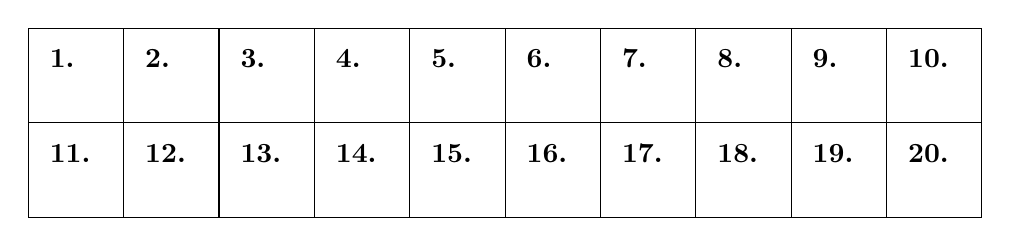
\begin{tikzpicture}
  % ---- 根据题数自动设置：16题为 8×2，20题为 10×2 ----
  \pgfmathtruncatemacro{\cols}{ifthenelse(\answerkeytotal<=16,8,10)}
  \pgfmathsetlengthmacro{\boxw}{(\linewidth-0.4pt)/\cols}
  \pgfmathsetlengthmacro{\boxh}{1.2cm}
  \pgfmathsetlengthmacro{\offset}{0.15cm}

  \foreach \num in {1,...,\answerkeytotal} {
    \pgfmathtruncatemacro{\row}{ifthenelse(\num<=\cols,0,1)}
    \pgfmathtruncatemacro{\col}{mod(\num-1,\cols)}
    \pgfmathsetlengthmacro{\x}{\col*\boxw}
    \pgfmathsetlengthmacro{\y}{-\row*\boxh}
    \draw (\x,\y) rectangle ++(\boxw,\boxh);
    \node[anchor=north west] at (\x+\offset,\y+\boxh-\offset) {\textbf{\num.}};
  }
\end{tikzpicture}

\end{flushleft}

%region 范围：初一（Form 1）基础几何 | 考点：平行四边形面积公式（底×高） | 难度：基础
\begin{question}
    如下图所示，平行四边形 $ABCD$ 中，底边 $AB = 8\text{ cm}$，一腰 $AD = 6\text{ cm}$，$AB$ 边上的高为 $5\text{ cm}$，则该平行四边形的面积为 
    \paren[C]


    \begin{center}
    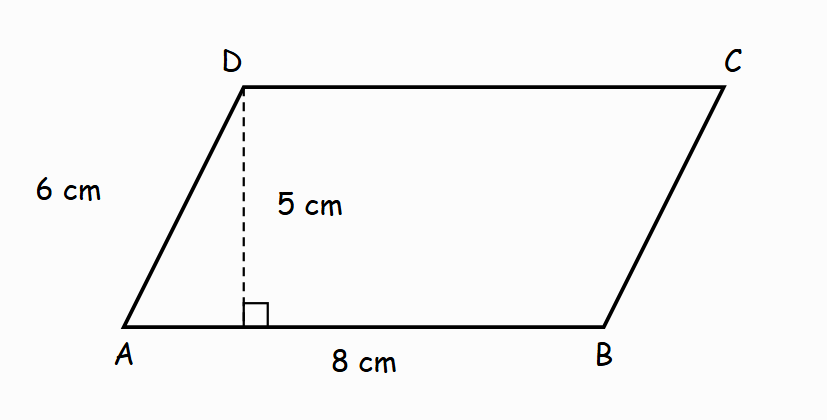
\includegraphics[width=0.5\textwidth]{AUG_J2_PAPER1/image.png}
    % \begin{tikzpicture}[scale=0.55]
    %     \coordinate (A) at (0,0);
    %     \coordinate (B) at (8,0);
    %     \coordinate (C) at (9.5,3);
    %     \coordinate (D) at (1.5,3);
    %     \coordinate (E) at (1.5,0);

    %     \draw[thick] (A) -- (B) -- (C) -- (D) -- cycle;
    %     \draw[dashed] (D) -- (E);
    %     \draw (1.5,0.3) -- (1.8,0.3) -- (1.8,0);

    %     \node[below] at ($(A)!0.5!(B)$) {$8\text{ cm}$};
    %     \node[left]  at ($(A)!0.5!(D)$) {$6\text{ cm}$};
    %     \node[right] at ($(D)!0.5!(E)$) {$5\text{ cm}$};

    %     \node[below left]  at (A) {$A$};
    %     \node[below right] at (B) {$B$};
    %     \node[above right] at (C) {$C$};
    %     \node[above left]  at (D) {$D$};
    % \end{tikzpicture}
    \end{center}

    \begin{choices}
        \item $20\text{ cm}^2$
        \item $28\text{ cm}^2$
        \item $40\text{ cm}^2$
        \item $48\text{ cm}^2$
    \end{choices}
\end{question}

\begin{solution}
    \textbf{解析：} \\
    平行四边形的面积公式为「底 $\times$ 高」，而非「底 $\times$ 腰长」。 \\
    题目给出底边 $AB = 8\text{ cm}$，且该底边上的高为 $5\text{ cm}$，代入公式：
    \[ \displaystyle S = AB \times h = 8 \times 5 = 40\ (\text{cm}^2) \]
    选项 D（$48\text{ cm}^2$）是误将腰长 $AD = 6\text{ cm}$ 当作高，计算 $8 \times 6$ 所致；\\
    选项 B（$28\text{ cm}^2$）是误用了周长公式 $(8+6)\times 2$；\\
    选项 A（$20\text{ cm}^2$）是误套用了三角形面积公式 $\dfrac{1}{2} \times 8 \times 5$。\\
    故选 C。
\end{solution}
%endregion

%region 范围：初中/高中几何 - 四边形性质 | 考点：对角线判别四边形类型 | 难度：基础
\begin{question}
    在凸四边形中，若对角线互相垂直且互相平分，则该四边形必为下列何种图形？ \paren[C]
    \begin{choices}
        \item 平行四边形
        \item 长方形
        \item 菱形
        \item 正方形
    \end{choices}
\end{question}

\begin{solution}
    \textbf{解析：} \\
    首先，对角线互相平分是判定四边形为平行四边形的充要条件之一，故该四边形必为平行四边形。 \\
    接着考察"对角线互相垂直"这一额外条件对平行四边形的限制：
    \[ \displaystyle \text{对角线垂直} \;\Longleftrightarrow\; \text{四条边长度相等（邻边相等的平行四边形）} \]
    这是因为对角线互相平分后，四个直角三角形的两条直角边（半对角线长）分别相同，
    对角线垂直使这四个直角三角形全等，从而四条边长必然相等，即为菱形的定义特征。 \\
    逐一排除干扰项：
    \begin{itemize}
        \item[A.] 平行四边形——仅由"对角线互相平分"即可得出，未用到"垂直"这一条件，条件不完整，排除。
        \item[B.] 矩形——矩形的判定条件是对角线互相平分且\textbf{相等}（而非垂直），
        与本题给出的垂直条件不符，排除。
        \item[D.] 正方形——正方形需同时满足对角线垂直、平分\textbf{且相等}，
        题目并未给出"相等"这一条件，因此不能确定为正方形，属于以偏概全的干扰项，排除。
    \end{itemize}
    综上，仅凭"对角线互相垂直且互相平分"这一条件，能唯一确定的图形是菱形。 \\
    故选 C。
\end{solution}
%endregion

%region 范围：初中几何 - 多边形内角和 | 考点：内角和公式逆用求边数 | 难度：基础
\begin{question}
    已知一个凸多边形的内角和为 $1620°$，求该多边形的边数。 \paren[C]
    \begin{choices}
        \item $9$
        \item $10$
        \item $11$
        \item $12$
    \end{choices}
\end{question}

\begin{solution}
    \textbf{解析：} \\
    多边形内角和公式为：
    \[ \displaystyle (n-2) \times 180° = a \]
    其中 $n$ 为边数，$a$ 为内角和。将已知条件 $a = 1620°$ 代入公式：
    \[ \displaystyle (n-2) \times 180° = 1620° \]
    两边同除以 $180°$：
    \[ \displaystyle n - 2 = \frac{1620}{180} = 9 \]
    解得：
    \[ \displaystyle n = 9 + 2 = 11 \]
    逐一排除干扰项：
    \begin{itemize}
        \item[A.] $9$——若误将 $\frac{1620}{180}$ 的商直接当作边数 $n$（忘记加 2），
        会得到 $n = 9$，属于漏用公式中"$-2$"项的常见计算失误。
        \item[B.] $10$——若在换算过程中出现除法或加法的一位数偏差
        （如误算 $\frac{1620}{180} = 8$ 后加 2），会得到此干扰值。
        \item[D.] $12$——若误将公式记成 $(n-1) \times 180° = a$（与三角形内角和 $180°$ 的记忆混淆，
        错误地多加了一条边），代入后会得到 $n = 12$，是公式记忆错误的典型干扰项。
    \end{itemize}
    故选 C。
\end{solution}
%endregion

% 范围：初中几何 - 正多边形 | 考点：外角和恒为360°、正多边形边数求解 | 难度：基础
%region 范围：初中几何 - 正多边形 | 考点：外角和恒为360°、正多边形边数求解 | 难度：基础
\begin{question}
    已知一个正多边形的每一个外角为 $24°$，求该正多边形的边数。 \paren[C]
    \begin{choices}
        \item $12$
        \item $13$
        \item $15$
        \item $18$
    \end{choices}
\end{question}

\begin{solution}
    \textbf{解析：} \\
    任意凸多边形的外角和恒为 $360°$，正多边形每个外角相等，故：
    \[ \displaystyle n = \frac{360°}{\text{每个外角}} \]
    代入每个外角 $24°$：
    \[ \displaystyle n = \frac{360°}{24°} = 15 \]
    逐一排除干扰项：
    \begin{itemize}
        \item[A.] $12$——误用内角和公式 $(n-2)\times180°=24°\times n$ 时代数变形出错所致。
        \item[B.] $13$——除法计算失误（如误算 $360\div24$ 时漏看余数为 $0$，凑整错误）。
        \item[D.] $18$——把 $24°$ 误当作内角而非外角代入 $(n-2)\times180°/n=24°$ 求解，方向搞反。
    \end{itemize}
    故选 C。
\end{solution}
%endregion

\newpage 


%region 范围：初一（Form 1）基础几何 | 考点：平行四边形与三角形面积公式的综合运用 | 难度：中等
\begin{question}
    如下图所示，梯形 $ABCD$ 由三角形 $ADE$ 与平行四边形 $EBCD$ 拼接而成，其中 $E$ 为 $AB$ 上一点。已知 $AE = 4\text{ cm}$，平行四边形 $EBCD$ 的底边 $EB = 6\text{ cm}$，其面积为 $30\text{ cm}^2$，则梯形 $ABCD$ 的面积为 \paren[B]

    \begin{center}
    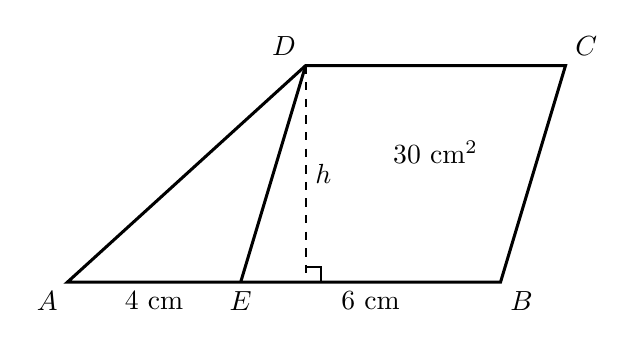
\begin{tikzpicture}[scale=0.55, every node/.style={font=\normalsize}]
        \coordinate (A) at (0,0);
        \coordinate (E) at (4,0);
        \coordinate (B) at (10,0);
        \coordinate (D) at (5.5,5);
        \coordinate (C) at (11.5,5);
        \coordinate (F) at (5.5,0);

        \draw[line width=1.1pt] (A) -- (B) -- (C) -- (D) -- cycle;
        \draw[line width=1.1pt] (E) -- (D);
        \draw[line width=0.8pt, dashed] (D) -- (F);
        \draw[line width=0.8pt] (5.5,0.35) -- (5.85,0.35) -- (5.85,0);

        \node[below] at ($(A)!0.5!(E)$) {$4\text{ cm}$};
        \node[below] at ($(E)!0.5!(B)$) {$6\text{ cm}$};
        \node at (8.5,3) {$30\text{ cm}^2$};
        \node[right] at (5.5,2.5) {$h$};

        \node[below left] at (A) {$A$};
        \node[below] at (E) {$E$};
        \node[below right] at (B) {$B$};
        \node[above right] at (C) {$C$};
        \node[above left] at (D) {$D$};
    \end{tikzpicture}
    \end{center}

    \begin{choices}
        \item $34\text{ cm}^2$
        \item $40\text{ cm}^2$
        \item $45\text{ cm}^2$
        \item $50\text{ cm}^2$
    \end{choices}
\end{question}

\begin{solution}
    \textbf{解析：} \\
    第一步，由平行四边形 $EBCD$ 的面积公式「底 $\times$ 高」求出高 $h$：
    \[ \displaystyle h = \frac{S_{EBCD}}{EB} = \frac{30}{6} = 5\ (\text{cm}) \]
    第二步，梯形的高处处相等，因此三角形 $ADE$ 的高也等于 $h = 5\text{ cm}$，其底边为 $AE = 4\text{ cm}$，代入三角形面积公式：
    \[ \displaystyle S_{ADE} = \frac{1}{2} \times AE \times h = \frac{1}{2} \times 4 \times 5 = 10\ (\text{cm}^2) \]
    第三步，梯形 $ABCD$ 由三角形 $ADE$ 与平行四边形 $EBCD$ 拼接而成，故：
    \[ \displaystyle S_{ABCD} = S_{ADE} + S_{EBCD} = 10 + 30 = 40\ (\text{cm}^2) \]
    选项 D（$50\text{ cm}^2$）是求三角形面积时漏乘 $\dfrac{1}{2}$，误算为 $4\times5+30$ 所致；\\
    选项 C（$45\text{ cm}^2$）是把三角形的底边当成了平行四边形的底来求高，误算 $h = 30\div4 = 7.5$，再代入三角形公式；\\
    选项 A（$34\text{ cm}^2$）是把三角形的边长直接当作面积相加，即 $30 + 4$，未经过任何面积计算。\\
    故选 B。
\end{solution}
%endregion


%region 范围：初中几何 | 考点：平行线性质、Z字型/拐点模型角度传递 | 难度：困难
\begin{question}
    如下图所示，已知AE//CD， BC//ED。求 $\angle x + \angle y$ 的度数。 \paren[C]
    
    \begin{center}
    \usetikzlibrary{decorations.markings, arrows.meta, quotes, angles, calc}
    \tikzset{
        mid arrow/.style={postaction={decorate,decoration={
            markings, mark=at position .6 with {\arrow[scale=1.2]{Latex}}
        }}},
        mid double arrow/.style={postaction={decorate,decoration={
            markings,
            mark=at position .53 with {\arrow[scale=1.2]{Latex}},
            mark=at position .63 with {\arrow[scale=1.2]{Latex}}
        }}}
    }
    \begin{tikzpicture}[scale=1]
        % 基准点
        \coordinate (A) at (0, 3.5);
        \coordinate (B) at ([shift={(-45:2.5)}]A);
        \coordinate (C) at ([shift={(43:3)}]B);
        \coordinate (E) at (0, -2);
        \coordinate (D) at (intersection of C--{[shift={(0,-5)}]C} and E--{[shift={(43:6)}]E});
        
        % 绘制左侧双箭头平行线
        \draw[thick] (0, 5) -- (A) -- (E) -- (0, -3.5);
        \draw[thick, mid double arrow] (0, 2) -- (0, -0.5);

        % 绘制右侧双箭头平行线 CD
        \draw[thick, mid double arrow] (C) -- (D);
        
        % 绘制单箭头平行线 BC 和 ED
        \draw[thick, mid arrow] (B) -- (C);
        \draw[thick, mid arrow] (E) -- (D);
        
        % 绘制连接线 AB
        \draw[thick] (A) -- (B);

        % 标注每一个点的字母
        \fill (A) circle (1.5pt) node[left=2pt] {$A$};
        \fill (B) circle (1.5pt) node[above=2pt] {$B$};
        \fill (C) circle (1.5pt) node[right=2pt] {$C$};
        \fill (D) circle (1.5pt) node[right=2pt] {$D$};
        \fill (E) circle (1.5pt) node[left=2pt] {$E$};

        % 统一使用 angle eccentricity=1.4 标注角度
        \coordinate (A_up) at (0, 4.5);
        \pic[draw, thick, angle radius=0.6cm, "$135^\circ$", angle eccentricity=1.8] {angle=B--A--A_up};
        \pic[draw, thick, angle radius=0.6cm, "$268^\circ$", angle eccentricity=1.4] {angle=A--B--C};
        \pic[draw, thick, angle radius=0.7cm, "$y$", angle eccentricity=1.4] {angle=B--C--D};
        \coordinate (E_up) at (0, -1);
        \pic[draw, thick, angle radius=0.7cm, "$x$", angle eccentricity=1.4] {angle=D--E--E_up};

    \end{tikzpicture}
    \end{center}

    \begin{choices}
        \item $86^\circ$
        \item $90^\circ$
        \item $94^\circ$
        \item $104^\circ$
    \end{choices}
\end{question}

\begin{solution}
    \textbf{解析：} \\
    步骤 1：梳理平行关系与初始角度。\\
    记最左侧的直线为直线 $AE$，右侧的线段为 $CD$。已知 $AE \parallel CD$。\\
    记图中标有单箭头的两线段分别为 $BC, ED$，已知 $BC \parallel ED$。\\
    图中拐点 $B$ 处的反射角为 $268^\circ$，则该拐点处位于图形内部的锐角为 $360^\circ - 268^\circ = 92^\circ$，即 $\angle ABC = 92^\circ$。

    步骤 2：利用平行线传递角度（求 $\angle y$）。\\
    过拐点 $B$ 作一条平行于 $AE$ 的辅助线 $BF$（向上方引射线）。\\
    $\because$ 辅助线 $BF \parallel AE$，\\
    $\therefore$ 根据同旁内角互补，可得 $\angle ABF = 180^\circ - 135^\circ = 45^\circ$。\\
    又 $\because$ 拐点内部的总角度 $\angle ABC = 92^\circ$，\\
    $\therefore \angle FBC = \angle ABC - \angle ABF = 92^\circ - 45^\circ = 47^\circ$。\\
    $\because$ 辅助线 $BF \parallel CD$（因为 $BF \parallel AE$ 且 $AE \parallel CD$），\\
    $\therefore$ 根据两直线平行，内错角相等，可得 $\angle y = \angle BCD = \angle FBC = 47^\circ$。

    步骤 3：利用平行线传递角度（求 $\angle x$）。\\
    $\because BC \parallel ED$，且它们分别与互相平行的 $AE, CD$ 相交，\\
    根据平行线的性质（同位角/内错角的多次传递），平行的线段与平行的直线所夹的锐角必然相等。\\
    由于 $\angle y$ 是 $BC$ 与 $CD$ 的夹角，$\angle x$ 是 $ED$ 与 $AE$ 的夹角，\\
    $\therefore \angle x = \angle y = 47^\circ$。

    步骤 4：计算最终结果。
    \[ \displaystyle \angle x + \angle y = 47^\circ + 47^\circ = 94^\circ \]
    选项 C 正确。\\
    故选 C。
\end{solution}
%endregion



\newpage

%region 范围：初中几何 | 考点：多边形内角和、外角定理、飞镖模型 | 难度：中等
\begin{question}
    如下图所示，下列哪项满足a,c,b,d之间的关系？ \paren[A]
    
    \begin{center}
    \usetikzlibrary{quotes, angles, calc}
    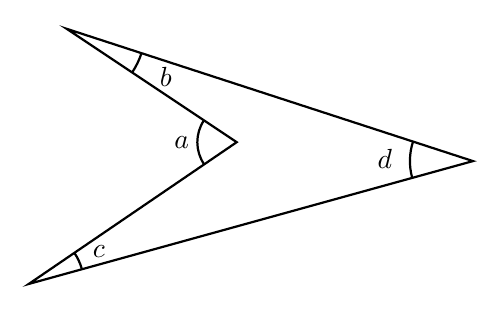
\begin{tikzpicture}[scale=1.2]
        % 定义顶点坐标
        \coordinate (A) at (0,0);       % 凹顶点
        \coordinate (B) at (-1.8, 1.2); % 左上顶点
        \coordinate (C) at (-2.2, -1.5);% 左下顶点
        \coordinate (D) at (2.5, -0.2); % 右侧顶点

        % 绘制四边形边界
        \draw[thick] (B) -- (A) -- (C) -- (D) -- cycle;

        % 标注角度 (统一使用 angle eccentricity=1.4)
        \pic[draw, thick, angle radius=0.5cm, "$a$", angle eccentricity=1.4] {angle=B--A--C};
        \pic[draw, thick, angle radius=1.0cm, "$b$", angle eccentricity=1.4] {angle=A--B--D};
        \pic[draw, thick, angle radius=0.7cm, "$c$", angle eccentricity=1.4] {angle=D--C--A};
        \pic[draw, thick, angle radius=0.8cm, "$d$", angle eccentricity=1.4] {angle=B--D--C};
    \end{tikzpicture}
    \end{center}

    \begin{choices}
        \item $a = b + c + d$
        \item $a + b + c + d = 360^\circ$
        \item $a = b + c - d$
        \item $a + b + c + d = 180^\circ$
    \end{choices}
\end{question}

\begin{solution}
    \textbf{解析：} \\
    步骤 1：分析图形特征。该图形为经典的“飞镖模型”（非凸四边形），求解凹顶点处的角度通常需要通过作辅助线构造三角形，利用“三角形的外角等于与它不相邻的两个内角之和”来推导。
    
    步骤 2：构造辅助线。连接右侧顶点与凹顶点，并向左侧延长交对边于点 $E$（或直接以射线形式延长）。
    
    \begin{center}
    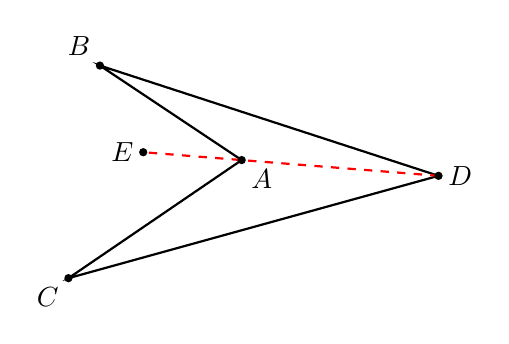
\begin{tikzpicture}[scale=1]
        \coordinate (A) at (0,0);
        \coordinate (B) at (-1.8, 1.2);
        \coordinate (C) at (-2.2, -1.5);
        \coordinate (D) at (2.5, -0.2);
        
        \draw[thick] (B) -- (A) -- (C) -- (D) -- cycle;
        
        % 辅助线
        \coordinate (E) at ($(D)!1.5!(A)$);
        \draw[dashed, red, thick] (D) -- (E);

        % 辅助点标注
        \fill (A) circle (1.5pt) node[below right] {$A$};
        \fill (B) circle (1.5pt) node[above left] {$B$};
        \fill (C) circle (1.5pt) node[below left] {$C$};
        \fill (D) circle (1.5pt) node[right] {$D$};
        \fill (E) circle (1.5pt) node[left] {$E$};
    \end{tikzpicture}
    \end{center}

    步骤 3：利用外角定理推导。\\
    在 $\triangle ABD$ 中，$\angle BAE$ 是 $\triangle ABD$ 的一个外角，\\
    $\therefore \angle BAE = \angle B + \angle BDA$。\\
    同理，在 $\triangle ACD$ 中，$\angle CAE$ 是 $\triangle ACD$ 的一个外角，\\
    $\therefore \angle CAE = \angle C + \angle CDA$。
    
    步骤 4：整合结论。\\
    由图可知，凹顶点处的角 $a = \angle BAC = \angle BAE + \angle CAE$。\\
    将上述两式相加可得：
    \[ \displaystyle a = (\angle B + \angle BDA) + (\angle C + \angle CDA) = \angle B + \angle C + (\angle BDA + \angle CDA) \]
    即 $a = \angle B + \angle C + \angle D$。\\
    对应题干中的符号，即 $a = b + c + d$。选项 A 正确，其余干扰项均未能正确掌握外角传递关系。\\
    故选 A。
\end{solution}
%endregion


%region 范围：初中几何 | 考点：平行线性质、三角形内角和、多边形角度计算 | 难度：中等
\begin{question}
    如下图所示，在梯形 $ABCD$ 中，$AD \parallel BC$。已知 $\angle BAD = 115^\circ$，$\angle BCD = 65^\circ$。连接对角线 $BD$，若 $\angle ABD = 45^\circ$，则 $\angle CDB$ 的度数为 \paren[C]
    
    \begin{center}
    \usetikzlibrary{quotes, angles, calc}
    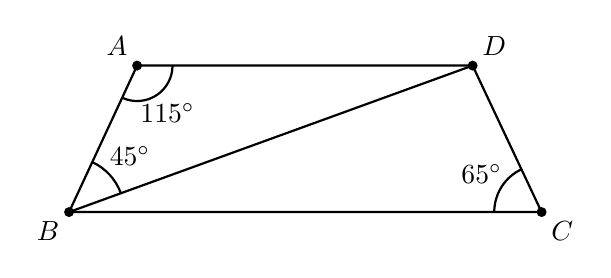
\begin{tikzpicture}[scale=1.2]
        % 根据真实角度计算的精确坐标
        % BC 放在 x 轴上，B 为原点 (0,0)
        \coordinate (B) at (0,0);
        \coordinate (C) at (5,0);
        
        % 角度 ABC = 180 - 115 = 65度。角度 DBC = 65 - 45 = 20度。
        % A 点位于 65 度的射线上，D 点位于 20 度的射线上，且 AD 平行于 BC (y坐标相同)
        % 通过几何计算得出 A 和 D 的近似坐标以保证按比例作图
        \coordinate (A) at (0.72, 1.55);
        \coordinate (D) at (4.27, 1.55);

        % 绘制梯形及对角线
        \draw[thick] (A) -- (B) -- (C) -- (D) -- cycle;
        \draw[thick] (B) -- (D);

        % 顶点标注
        \fill (A) circle (1.5pt) node[above left] {$A$};
        \fill (B) circle (1.5pt) node[below left] {$B$};
        \fill (C) circle (1.5pt) node[below right] {$C$};
        \fill (D) circle (1.5pt) node[above right] {$D$};

        % 角度标注 (统一使用 angle eccentricity=1.4)
        \pic[draw, thick, angle radius=0.45cm, "$115^\circ$", angle eccentricity=1.6] {angle=B--A--D};
        \pic[draw, thick, angle radius=0.6cm, "$65^\circ$", angle eccentricity=1.5] {angle=D--C--B};
        \pic[draw, thick, angle radius=0.7cm, "$45^\circ$", angle eccentricity=1.5] {angle=D--B--A};
    \end{tikzpicture}
    \end{center}

    \begin{choices}
        \item $45^\circ$
        \item $50^\circ$
        \item $95^\circ$
        \item $115^\circ$
    \end{choices}
\end{question}

\begin{solution}
    \textbf{解析：} \\
    步骤 1：利用平行线的同旁内角互补关系求 $\angle ABC$。\\
    $\because AD \parallel BC$，\\
    $\therefore \angle ABC + \angle BAD = 180^\circ$。\\
    又 $\because \angle BAD = 115^\circ$，\\
    $\therefore \angle ABC = 180^\circ - 115^\circ = 65^\circ$。

    步骤 2：利用角度差求 $\angle DBC$。\\
    $\because \angle ABC = 65^\circ$，且已知对角线 $BD$ 将其分割使得 $\angle ABD = 45^\circ$，\\
    $\therefore \angle DBC = \angle ABC - \angle ABD = 65^\circ - 45^\circ = 20^\circ$。

    步骤 3：在 $\triangle BCD$ 中利用内角和求目标角度。\\
    在 $\triangle BCD$ 中，已知 $\angle BCD = 65^\circ$，且刚求得 $\angle DBC = 20^\circ$。\\
    根据三角形内角和定理：
    \[ \displaystyle \angle CDB = 180^\circ - \angle BCD - \angle DBC = 180^\circ - 65^\circ - 20^\circ = 95^\circ \]
    
    （注：也可通过平行线内错角 $\angle ADB = \angle DBC = 20^\circ$，同旁内角 $\angle ADC = 180^\circ - 65^\circ = 115^\circ$，再由 $\angle CDB = \angle ADC - \angle ADB$ 求得，结果一致。）

    步骤 4：干扰项分析。\\
    选项 A 错误，误将 $\angle ABD$ 和 $\angle CDB$ 当作平行线的内错角；\\
    选项 D 错误，误判四边形为平行四边形导致对角相等；\\
    正确计算结果为 $95^\circ$。\\
    故选 C。
\end{solution}
%endregion

% 范围：小学数学/初等几何 | 考点：图形面积计算与面积单位（平方千米）换算 | 难度：中等
\begin{question}
    如下图所示，某城市规划了一块矩形硬化场地用于建设大型市民广场。已知该矩形场地的长为 $500 \, \mathrm{m}$，宽为 $400 \, \mathrm{m}$。请问这块场地的面积是?\paren[A]
    
    \begin{center}
    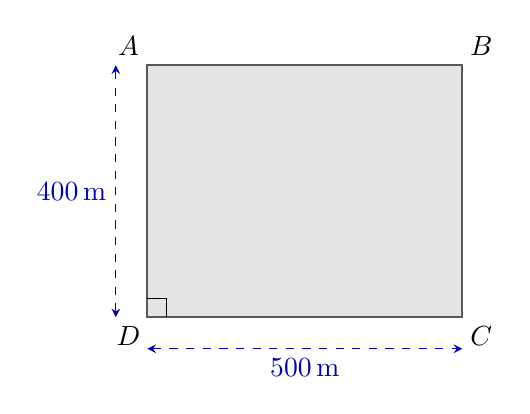
\begin{tikzpicture}[scale=0.8, >=stealth]
        % 绘制带背景色的矩形，颜色按要求改为灰色
        \draw[thick, fill=gray!20, draw=gray!70!black] (0,0) rectangle (5,4);
        
        % 标注边长
        \draw[<->, dashed, blue!70!black] (0,-0.5) -- (5,-0.5) node[midway, below] {$500 \, \mathrm{m}$};
        \draw[<->, dashed, blue!70!black] (-0.5,0) -- (-0.5,4) node[midway, left] {$400 \, \mathrm{m}$};
        
        % 顶点直角符号标注
        \draw (0.3,0) -- (0.3,0.3) -- (0,0.3);
        
        % 顶点字母 (增加学术感)
        \node at (-0.3, 4.3) {$A$};
        \node at (5.3, 4.3) {$B$};
        \node at (5.3, -0.3) {$C$};
        \node at (-0.3, -0.3) {$D$};
    \end{tikzpicture}
    \end{center}

    \begin{choices}
        \item $0.2 \, \mathrm{km}^2$
        \item $2 \, \mathrm{km}^2$
        \item $20 \, \mathrm{km}^2$
        \item $200000 \, \mathrm{km}^2$
    \end{choices}
\end{question}

\begin{solution}
    \textbf{解析：} \\
    步骤 1：分析题意与知识点引入。 \\
    本题结合了基础几何图形（矩形）的面积计算与高级面积单位（平方千米）的换算。我们需要先求出场地的面积（以 $\mathrm{m}^2$ 为单位），再利用 $1 \, \mathrm{km}^2 = 1000000 \, \mathrm{m}^2$ 的进率进行单位换算。 \\
    
    步骤 2：公式计算与推导验证。 \\
    首先，根据矩形面积公式 $S = \text{长} \times \text{宽}$，计算场地的实际面积：
    \[ \displaystyle S = 500 \, \mathrm{m} \times 400 \, \mathrm{m} = 200000 \, \mathrm{m}^2 \]
    接着，将平方米换算为平方千米。由低级单位向高级单位转换，需除以进率 $1000000$：
    \[ \displaystyle \text{目标面积} = \frac{200000}{1000000} \, \mathrm{km}^2 = 0.2 \, \mathrm{km}^2 \]
    
    步骤 3：结论梳理与干扰项排查。 \\
    经过严密计算，实际面积为 $0.2 \, \mathrm{km}^2$，对应选项 A。 
    \begin{itemize}
        \item 选项 B（$2 \, \mathrm{km}^2$）：错将换算进率记为 $100000$ 导致结果扩大 $10$ 倍。
        \item 选项 C（$20 \, \mathrm{km}^2$）：错将进率当成 $10000$（混淆了公顷的进率），导致结果扩大 $100$ 倍。
        \item 选项 D（$200000 \, \mathrm{km}^2$）：求出基本面积后，完全忘记进行单位换算，未区分平方米与平方千米。
    \end{itemize} 
    
    故选 A。
\end{solution}

\newpage

%region 范围：初中/高中几何 - 风筝形（鸢形）性质 | 考点：邻边相等四边形的对角相等性质、四边形内角和 | 难度：中等
% 注：本题 TikZ 需要 \usetikzlibrary{quotes,angles}
\begin{question}
    如下图所示，四边形 $ABCD$ 为风筝形，其中 $AB = AD$，$CB = CD$
    已知 $\angle BAD = 90°$，$\angle BCD = 60°$，求 $\angle ABC$ 的值。
\begin{center}
        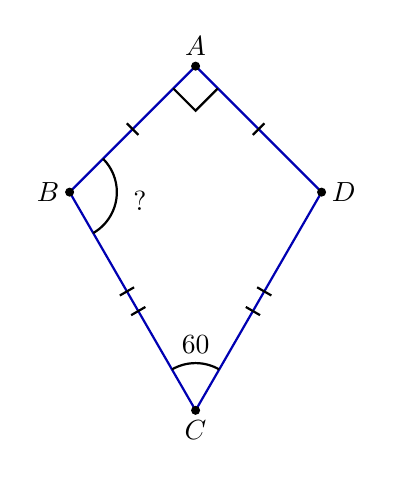
\begin{tikzpicture}[scale=0.8, >=stealth, thick]
        \coordinate (A) at (0, 2);
        \coordinate (B) at (-2, 0);
        \coordinate (C) at (0, -3.464);
        \coordinate (D) at (2, 0);

        \draw[thick, blue!70!black] (A) -- (B) -- (C) -- (D) -- cycle;

        % 单撇：AB、AD 等长标记
        \draw (-1.092,1.092) -- (-0.908,0.908);
        \draw (0.908,0.908) -- (1.092,1.092);

        % 双撇：CB、CD 等长标记
        \draw (-0.797,-1.823) -- (-1.023,-1.953);
        \draw (-0.977,-1.511) -- (-1.203,-1.641);
        \draw (1.023,-1.953) -- (0.797,-1.823);
        \draw (1.203,-1.641) -- (0.977,-1.511);

        \pic [draw, angle radius=4mm] {right angle = D--A--B};
        \pic [draw, "$60°$", angle eccentricity=1.4, angle radius=6mm] {angle = D--C--B};
        \pic [draw, "?", angle eccentricity=1.5, angle radius=6mm] {angle = C--B--A};

        \filldraw (A) circle (1.5pt) node[above] {$A$};
        \filldraw (B) circle (1.5pt) node[left] {$B$};
        \filldraw (C) circle (1.5pt) node[below] {$C$};
        \filldraw (D) circle (1.5pt) node[right] {$D$};
    \end{tikzpicture} \paren[B]
\end{center}

    \begin{choices}
        \item $75°$
        \item $105°$
        \item $135°$
        \item $210°$
    \end{choices}
\end{question}

\begin{solution}
    \textbf{解析：} \\
    风筝形（鸢形）中，两组邻边相等（$AB=AD$，$CB=CD$）会导致夹在两组不等边之间的一对对角相等，
    即 $\angle ABC = \angle ADC$（本题即所求角与其对角相等，但两者数值未知，仍需借助角度和求解）。 \\
    四边形内角和恒为 $360°$：
    \[ \displaystyle \angle BAD + \angle BCD + \angle ABC + \angle ADC = 360° \]
    代入 $\angle ABC = \angle ADC$（设为 $x$）及已知角：
    \[ \displaystyle 90° + 60° + 2x = 360° \]
    \[ \displaystyle 2x = 360° - 150° = 210° \]
    \[ \displaystyle x = 105° \]
    逐一排除干扰项：
    \begin{itemize}
        \item[D.] $210°$——求出 $2x=210°$ 后忘记再除以 $2$，直接把 $210°$ 当作答案。
        \item[C.] $135°$——只减去 $\angle BAD=90°$，漏减 $\angle BCD=60°$，即误算 $\dfrac{360°-90°}{2}=135°$。
        \item[A.] $75°$——误把性质记反，以为 $\angle ABC+\angle ADC = \angle BAD+\angle BCD$（本应是对角关系而非邻角关系），
        算出 $\dfrac{90°+60°}{2}=75°$，属于对角/邻角关系混淆的典型错误。
    \end{itemize}
    故选 B。
\end{solution}

%endregion



%region 范围：初中数学/初等几何 | 考点：矩形性质、弧长计算、组合图形周长 | 难度：中等
\begin{question}
    如下图所示，在矩形 $ABCD$ 中，已知 $AB=4$，$BC=6$。以点 $A$ 为圆心，以矩形的短边 $AB$ 长为半径作 $\dfrac{1}{4}$ 圆弧，交 $AD$ 于点 $E$。求图中阴影部分的周长。（取 $\displaystyle \pi = \frac{22}{7}$） \paren[B]
    
    \begin{center}
    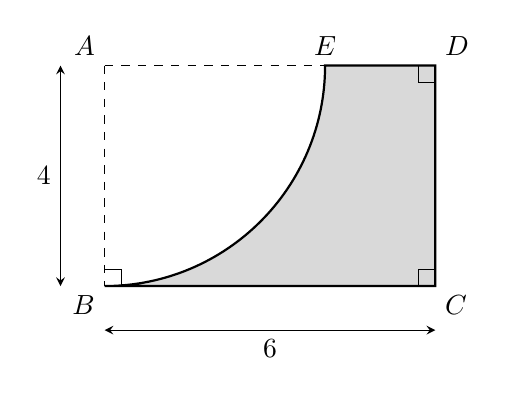
\begin{tikzpicture}[scale=0.7, >=stealth]
        % 变量定义
        \def\AB{4} % 短边
        \def\BC{6} % 长边
        
        % 顶点坐标
        \coordinate (A) at (0,\AB);
        \coordinate (B) at (0,0);
        \coordinate (C) at (\BC,0);
        \coordinate (D) at (\BC,\AB);
        \coordinate (E) at (\AB,\AB);
        
        % 绘制阴影区域 (矩形减去扇形 ABE)
        \draw[thick, fill=gray!30] (0,0) -- (\BC,0) -- (\BC,\AB) -- (\AB,\AB) arc (0:-90:\AB) -- cycle;
        
        % 绘制矩形剩余边界（无阴影部分）
        \draw[dashed, thin] (0,\AB) -- (\AB,\AB);
        \draw[dashed, thin] (0,\AB) -- (0,0);
        
        % 标注顶点
        \node[above left] at (A) {$A$};
        \node[below left] at (B) {$B$};
        \node[below right] at (C) {$C$};
        \node[above right] at (D) {$D$};
        \node[above] at (E) {$E$};
        
        % 标注边长
        \draw[<->] (-0.8, 0) -- (-0.8, \AB) node[midway, left] {$4$};
        \draw[<->] (0, -0.8) -- (\BC, -0.8) node[midway, below] {$6$};
        
        % 标注直角
        \draw (0, 0.3) -- (0.3, 0.3) -- (0.3, 0);
        \draw (\BC-0.3, 0) -- (\BC-0.3, 0.3) -- (\BC, 0.3);
        \draw (\BC, \AB-0.3) -- (\BC-0.3, \AB-0.3) -- (\BC-0.3, \AB);
        
    \end{tikzpicture}
    \end{center}

    \begin{choices}
        \item $\displaystyle \frac{100}{7}$
        \item $\displaystyle \frac{128}{7}$
        \item $\displaystyle \frac{142}{7}$
        \item $\displaystyle \frac{156}{7}$
    \end{choices}
\end{question}

\begin{solution}
    \textbf{解析：} \\
    步骤 1：分析图形组成与关键数据。 \\
    由题意知，四边形 $ABCD$ 为矩形，$\angle A = 90^\circ$，$AB=4$（短边），$BC=6$（长边）。
    根据矩形的对边相等性质，可知 $AD = BC = 6$，$CD = AB = 4$。
    以 $A$ 为圆心，$AB$ 为半径作 $\frac{1}{4}$ 圆弧，则扇形半径 $R = AB = 4$，且圆弧交 $AD$ 于点 $E$，所以 $AE = AB = 4$。 \\
    
    步骤 2：分析阴影部分周长的构成。 \\
    观察图形，阴影部分的边界是一个封闭图形，由以下四部分组成：
    1. 线段 $BC$；
    2. 线段 $CD$；
    3. 线段 $DE$；
    4. 圆弧 $\wideparen{BE}$。 \\
    
    步骤 3：计算各部分长度（注意按要求取 $\displaystyle \pi = \frac{22}{7}$）。 \\
    \begin{itemize}
        \item $BC = 6$；
        \item $CD = 4$；
        \item $DE = AD - AE = 6 - 4 = 2$；
        \item 弧 $\wideparen{BE}$ 的长度：由于 $\angle A = 90^\circ$，此弧为整个圆周的 $\frac{1}{4}$，
        \[ \displaystyle l_{\wideparen{BE}} = \frac{1}{4} \times 2 \pi R = \frac{1}{2} \times \frac{22}{7} \times 4 = \frac{44}{7} \]
    \end{itemize}
    
    步骤 4：汇总求和。 \\
    阴影部分的周长 $C = BC + CD + DE + l_{\wideparen{BE}}$：
    \[ \displaystyle C = 6 + 4 + 2 + \frac{44}{7} = 12 + \frac{44}{7} = \frac{84}{7} + \frac{44}{7} = \frac{128}{7} \]
    
    步骤 5：结论梳理与干扰项排查。 \\
    经过计算，阴影部分的周长为 $\displaystyle \frac{128}{7}$，对应选项 B。
    \begin{itemize}
        \item 选项 A（$\displaystyle \frac{100}{7}$）：计算直线部分时漏掉了线段 $DE$（即 $6+4+\frac{44}{7}$），对图形边界封闭性分析不全。
        \item 选项 D（$\displaystyle \frac{156}{7}$）：错误地将未被截取前的矩形长边 $AD$ 完整计算在内（即 $6+4+6+\frac{44}{7}$），忽略了扇形占据的空间。
        \item 选项 C（$\displaystyle \frac{142}{7}$）：直线部分计算错误，可能误将 $DE$ 的长度当作 $4$ 进行计算（即 $6+4+4+\frac{44}{7}$）。
    \end{itemize}
    
    故选 B。
\end{solution}
%endregion



%region 范围：初中数学/初等几何 | 考点：扇形面积公式及其逆运算 | 难度：中等
\begin{question}
    如下图所示，以O为圆心的扇形 $AOB$ 的圆心角 $\angle AOB = 120^\circ$。已知该扇形的面积为 $12\pi$，求扇形的半径。 \paren[B]
    
    \begin{center}
    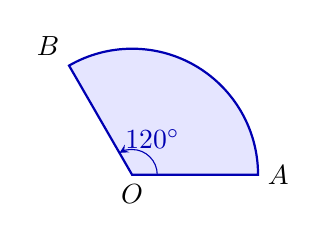
\begin{tikzpicture}[scale=0.8, >=stealth]
        % 绘制扇形并填充背景色
        \draw[thick, fill=blue!10, draw=blue!70!black] (0,0) -- (0:2) arc (0:120:2) -- cycle;
        
        % 绘制圆心角标记
        \draw[->, blue!70!black] (0.4,0) arc (0:120:0.4);
        \node[blue!70!black] at (60:0.65) {$120^\circ$};
        
        % 标注顶点字母
        \node[below] at (0,0) {$O$};
        \node[right] at (2,0) {$A$};
        \node[above left] at (120:2) {$B$};
        
        % % 标注半径
        % \node[below] at (1,0) {$r$};
    \end{tikzpicture}
    \end{center}

    \begin{choices}
        \item $3$
        \item $6$
        \item $18$
        \item $36$
    \end{choices}
\end{question}

\begin{solution}
    \textbf{解析：} \\
    步骤 1：分析题意与知识点引入。 \\
    本题考查扇形面积公式的逆向应用。已知扇形的中心角 $n = 120^\circ$ 以及扇形的面积 $S = 12\pi$，要求圆的半径 $r$。我们需要利用度数制下的扇形面积公式进行方程求解。扇形面积公式为：
    \[ \displaystyle S = \frac{n \pi r^2}{360} \]
    
    步骤 2：公式计算与推导验证。 \\
    将已知条件代入上述公式，构建关于半径 $r$ 的方程：
    \[ \displaystyle 12\pi = \frac{120 \cdot \pi \cdot r^2}{360} \]
    对等式右侧的系数进行约分化简：
    \[ \displaystyle 12\pi = \frac{1}{3}\pi r^2 \]
    等式两边同时消去 $\pi$，并同乘 $3$，解得 $r^2$：
    \[ \displaystyle r^2 = 36 \]
    因为半径 $r$ 表示线段长度，必须为正数，故对两边开平方得：
    \[ \displaystyle r = 6 \]
    
    步骤 3：结论梳理与干扰项排查。 \\
    经过计算，圆的半径为 $6$，对应选项 B。 
    \begin{itemize}
        \item 选项 A（$3$）：在解得 $r^2 = 36$ 后，错误地将开平方运算理解为了除以 $12$（误以为 $36 \div 12 = 3$），或在约分时发生计算失误。
        \item 选项 C（$18$）：错将扇形面积公式与弧长公式 $l = \frac{n\pi r}{180}$ 混淆，列出错误方程 $12\pi = \frac{120\pi r}{180}$，从而解出 $r = 18$。
        \item 选项 D（$36$）：解出 $r^2 = 36$ 后，忘记对结果进行开平方运算，直接将 $r^2$ 的值作为半径的最终答案。
    \end{itemize} 
    
    故选 B。
\end{solution}
%endregion

% 范围：初中代数 - 代数式求值 | 考点：整式运算、代入求值 | 难度：基础
\begin{question}
    已知 $x = -2$，$y = 3$，求代数式 $2x^2 - 3xy + y^2$ 的值。 \paren[D]
    \begin{choices}
        \item $-1$
        \item $19$
        \item $31$
        \item $35$
    \end{choices}
\end{question}

\begin{solution}
    \textbf{解析：} \\
    将 $x = -2$，$y = 3$ 代入原式：
    \[ \displaystyle 2x^2 - 3xy + y^2 = 2(-2)^2 - 3(-2)(3) + (3)^2 \]
    逐项计算：$2(-2)^2 = 2 \times 4 = 8$；$-3(-2)(3) = 18$；$(3)^2 = 9$ \\
    \[ \displaystyle = 8 + 18 + 9 = 35 \]
    逐一排除干扰项：
    \begin{itemize}
        \item[A.] $-1$——误把 $x = -2$ 当作 $x = 2$ 代入 $xy$ 项（平方项不受影响，但交叉项符号算错）。
        \item[C.] $31$——漏写系数，将 $2x^2$ 误算成 $x^2 = 4$，导致结果偏小 $4$。
        \item[B.] $19$——误将 $2x^2$ 算成 $-2x^2 = -8$（把 $x$ 的负号错误带入平方项）。
    \end{itemize}
    故选 D。
\end{solution}

% 范围：初中代数 - 乘法公式与化简 | 考点：平方差公式的逆用 | 难度：中等
\begin{question}
    化简 $(2x+3)^2 - (2x-3)^2$。 \paren[A]
    \begin{choices}
        \item $24x$
        \item $12x$
        \item $8x^2 + 18$
        \item $4x^2 - 12$
    \end{choices}
\end{question}

\begin{solution}
    \textbf{解析：} \\
    利用平方差公式 $a^2 - b^2 = (a+b)(a-b)$，设 $a = 2x+3$，$b = 2x-3$：
    \[ \displaystyle a + b = (2x+3)+(2x-3) = 4x, \qquad a - b = (2x+3)-(2x-3) = 6 \]
    代入公式：
    \[ \displaystyle (2x+3)^2 - (2x-3)^2 = 4x \times 6 = 24x \]
    逐一排除干扰项：
    \begin{itemize}
        \item[B.] $12x$——计算 $a-b$ 时符号处理错误，误得 $a-b=3$ 而非 $6$。
        \item[C.] $8x^2+18$——把减法误当加法，实际算出的是 $(2x+3)^2+(2x-3)^2$。
        \item[D.] $4x^2-12$——未使用公式，直接展开时漏项或漏乘，属于展开不完整的典型错误。
    \end{itemize}
    故选 A。
\end{solution}

%region 范围：信息科学与初等代数 | 考点：二进制混合四则运算 | 难度：中等
\begin{question}
    计算 $[1101_{2} \times 11_{2}] - 1010_{2}$ 的值。 \paren[C]
    
    \begin{choices}
        \item $10111_{2}$
        \item $11011_{2}$
        \item $11101_{2}$
        \item $11111_{2}$
    \end{choices}
\end{question}

\begin{solution}
    \textbf{解析：} \\
    步骤 1：进行二进制乘法运算。\\
    计算 $1101_{2} \times 11_{2}$：
    \[
    \begin{array}{r@{\quad}l}
    1101 & {} \\
    \times \phantom{00} 11 & {} \\
    \hline
    1101 & {} \\
    + \phantom{} 11010 & {} \\
    \hline
    100111 & {}
    \end{array}
    \]
    所以，$1101_{2} \times 11_{2} = 100111_{2}$。我们可以通过转换为十进制进行验证：$1101_{2} = 13_{10}$，$11_{2} = 3_{10}$，两者相乘为 $13 \times 3 = 39_{10}$。而 $100111_{2} = 32 + 4 + 2 + 1 = 39_{10}$，计算正确。

    步骤 2：进行二进制减法运算。\\
    计算 $100111_{2} - 1010_{2}$：
    \[
    \begin{array}{r@{\quad}l}
    100111 & {} \\
    - \phantom{00} 1010 & {} \\
    \hline
    11101 & {}
    \end{array}
    \]
    所以，最终结果为 $11101_{2}$。转换为十进制验证：$39_{10} - 1010_{2} = 39_{10} - 10_{10} = 29_{10}$。而 $11101_{2} = 16 + 8 + 4 + 1 = 29_{10}$，计算正确。

    步骤 3：干扰项分析。\\
    选项 B（$11011_{2}$ 为 $27_{10}$）和选项 A（$10111_{2}$ 为 $23_{10}$）均为在减法借位时出现计算失误导致的错误结果；\\
    选项 D（$11111_{2}$ 为 $31_{10}$）为直接将乘积错误算作 $101001_{2}$ 导致的偏差。\\
    
    故选 C。
\end{solution}
%endregion

%region 范围：信息科学与初等代数 | 考点：二进制与八进制的快捷转换 | 难度：中等
\begin{question}
    将二进数 $11010111_{2}$ 转换为八进数，其结果为 \paren[B]
    
    \begin{choices}
        \item $227_{8}$
        \item $327_{8}$
        \item $357_{8}$
        \item $657_{8}$
    \end{choices}
\end{question}

\begin{solution}
    \textbf{解析：} \\
    步骤 1：分析转换原理。\\
    由于 $2^3 = 8$，因此在进行二进制与八进制转换时，可采用“三位一体”法（又称 $4-2-1$ 规则），即以小数点为界，向左（和向右）每三位二进制数分为一组，不足三位时在高位补 $0$。

    步骤 2：分组并进行转换。\\
    将二进制数 $11010111_{2}$ 从右往左每三位进行分组：
    \[ \displaystyle \underline{011} \ \underline{010} \ \underline{111}_{2} \]
    (注意：最左侧的 $11$ 只有两位，在高位补 $0$ 得到 $011$)。\\
    将每组二进制数分别转换成对应的八进制数字：
    \begin{itemize}
        \item $\underline{011}_{2} = 0 \times 4 + 1 \times 2 + 1 \times 1 = 3_8$
        \item $\underline{010}_{2} = 0 \times 4 + 1 \times 2 + 0 \times 1 = 2_8$
        \item $\underline{111}_{2} = 1 \times 4 + 1 \times 2 + 1 \times 1 = 7_8$
    \end{itemize}
    将这三个八进制数字按顺序连接起来，即得到 $327_{8}$。

    步骤 3：干扰项分析。\\
    选项 D（$657_{8}$）是由于错误地从左往右进行分组：$\underline{110} \ \underline{101} \ \underline{11}_{2} \rightarrow 653_{8}$ 并伴随个位转化错误而产生的典型混淆项；\\
    选项 C（$357_{8}$）是在转化中间组 $\underline{010}_{2}$ 时将其错误地视为了 $5$；\\
    选项 A（$227_{8}$）则是高位分组 $011_{2}$ 计算失误，误将其当作 $2$。\\
    
    故选 B。
\end{solution}
%endregion

%region 范围：初中数学 - 计数制度 | 考点：八进制转十进制 | 难度：基础
\begin{question}
    将八进数 $367_{8}$ 转换为十进数，其结果为 \paren[B]
    \begin{choices}
        \item $237$
        \item $247$
        \item $257$
        \item $367$
    \end{choices}
\end{question}

\begin{solution}
    \textbf{解析：} \\
    八进制数各位数字按权重展开，权重从右到左依次为 $8^0, 8^1, 8^2, \ldots$ \\
    $(367)_8$ 展开为：
    \[ \displaystyle (367)_8 = 3 \times 8^2 + 6 \times 8^1 + 7 \times 8^0 \]
    逐项计算：
    \[ \displaystyle 3 \times 64 = 192, \qquad 6 \times 8 = 48, \qquad 7 \times 1 = 7 \]
    相加：
    \[ \displaystyle 192 + 48 + 7 = 247 \]
    $\therefore (367)_8 = (247)_{10}$ \\
    逐一排除干扰项：
    \begin{itemize}
        \item[A.] $237$——把最右一位 $7$ 的权重误算为 $8^0=1$ 没错，但十位（$6\times8$）算成了 $38$（乘法失误），
        导致 $192+38+7=237$。
        \item[C.] $367$——直接把八进制数字照抄当作十进制数值，完全忽略了进位制转换需要按权重展开的规则。
        \item[D.] $257$——把百位权重 $8^2=64$ 误记成 $8^2=70$ 附近的数值代入（权重记错），
        导致百位计算偏大。
    \end{itemize}
    故选 B。
\end{solution}
%endregion

%region 范围：初中几何 - 三角形面积 | 考点：钝角三角形面积、辨别有效数据 | 难度：中等偏难
\begin{question}
    如下图所示，$\triangle ABC$ 中 $\angle ABC$ 为钝角，$BC$ 边上的高为 $AD$（$D$ 落在 $BC$ 的延长线外）。
    已知 $BC = 12$ cm，$AD = 8$ cm，$AB = 10$ cm，求 $\triangle ABC$ 的面积。

    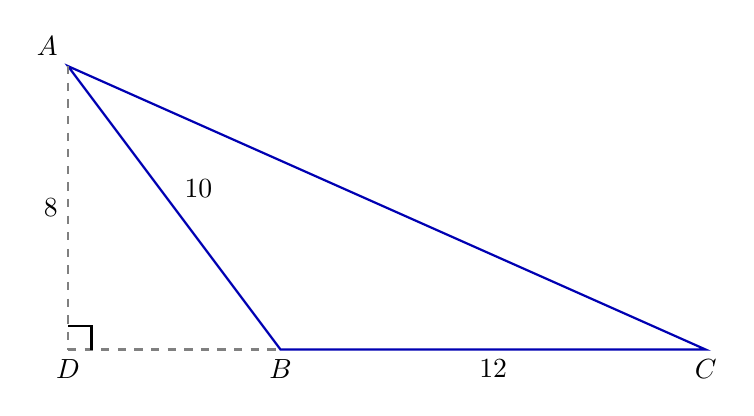
\begin{tikzpicture}[scale=0.45, >=stealth, thick]
        \coordinate (D) at (0,0);
        \coordinate (B) at (6,0);
        \coordinate (C) at (18,0);
        \coordinate (A) at (0,8);

        \draw[thick, blue!70!black] (A) -- (B) -- (C) -- cycle;
        \draw[dashed, gray] (A) -- (D);
        \draw[dashed, gray] (D) -- (B);
        \pic [draw, angle radius=3mm] {right angle = C--D--A};

        \node[above left] at (A) {$A$};
        \node[below] at (D) {$D$};
        \node[below] at (B) {$B$};
        \node[below] at (C) {$C$};

        \node[left] at ($(A)!0.5!(D)$) {$8$};
        \node[below] at ($(B)!0.5!(C)$) {$12$};
        \node[above right] at ($(A)!0.5!(B)$) {$10$};
    \end{tikzpicture} \paren[B]
    \begin{choices}
        \item $40$ cm$^2$
        \item $48$ cm$^2$
        \item $60$ cm$^2$
        \item $72$ cm$^2$
    \end{choices}
\end{question}

\begin{solution}
    \textbf{解析：} \\
    三角形面积公式只需底边及其对应的高：
    \[ \displaystyle S = \frac{1}{2} \times \text{底} \times \text{高} \]
    题目所求的是 $\triangle ABC$（底边 $BC$）的面积，$BC$ 边上对应的高为 $AD$，
    与 $BC$ 本身不共线的斜边 $AB=10$ 并非该面积公式所需的数据，属于多余的干扰条件。 \\
    代入 $\text{底}=BC=12$，$\text{高}=AD=8$：
    \[ \displaystyle S = \frac{1}{2} \times 12 \times 8 = \frac{96}{2} = 48 \text{ cm}^2 \]
    逐一排除干扰项：
    \begin{itemize}
        \item[A.] $40$ cm$^2$——误把斜边 $AB=10$ 当作底边代入，算成 $\dfrac{1}{2}\times10\times8=40$，
        没有意识到 $AB$ 与所求面积公式无关。
        \item[D.] $72$ cm$^2$——误以为底边应包含延长部分 $DB$，把 $DC = DB+BC = 6+12=18$ 当作底边，
        算成 $\dfrac{1}{2}\times18\times8=72$，混淆了"底边 $BC$"与"高的垂足到 $C$ 的距离"。
        \item[C.] $60$ cm$^2$——把高 $AD=8$ 误用斜边 $AB=10$ 代替，算成 $\dfrac{1}{2}\times12\times10=60$，
        属于"底"与"高"两个量分别代错数据的复合型错误。
    \end{itemize}
    故选 B。
\end{solution}
%endregion

% 范围：初中数学 - 计数制度 | 考点：十进制转二进制 | 难度：基础
%region 范围：初中数学 - 计数制度 | 考点：十进制转二进制（除2取余法） | 难度：基础
\begin{question}
    将十进数 $45_{10}$ 转换为二进数，其结果为 \paren[B]
    \begin{choices}
        \item $100101_{2}$
        \item $101101_{2}$
        \item $101110_{2}$
        \item $110101_{2}$
    \end{choices}
\end{question}

\begin{solution}
    \textbf{解析：} \\
    采用"除 $2$ 取余法"，将 $45$ 反复除以 $2$ 并记录余数，直至商为 $0$：
    \[ \displaystyle 45 \div 2 = 22 \cdots 1, \quad 22 \div 2 = 11 \cdots 0, \quad 11 \div 2 = 5 \cdots 1 \]
    \[ \displaystyle 5 \div 2 = 2 \cdots 1, \quad 2 \div 2 = 1 \cdots 0, \quad 1 \div 2 = 0 \cdots 1 \]
    将所得余数由下往上（即由最后一次到第一次）排列：
    \[ \displaystyle 45_{10} = 101101_{2} \]
    验证：$1{\times}32+0{\times}16+1{\times}8+1{\times}4+0{\times}2+1{\times}1 = 32+8+4+1=45$，正确。 \\
    逐一排除干扰项：
    \begin{itemize}
        \item[C.] $101110_{2}$——末两位余数顺序记反（$1$ 与 $0$ 互换），属于余数排列顺序错误。
        \item[A.] $100101_{2}$——中间某一步除法商或余数算错（如漏掉一次 $\div 2$ 的余数 $1$），导致对应的 $8$ 那一位错标为 $0$。
        \item[D.] $110101_{2}$——把最高位余数算错（多算一次商为 $1$ 的步骤），导致 $32$ 位与 $16$ 位同时被误标为 $1$。
    \end{itemize}
    故选 B。
\end{solution}
%endregion

\newpage
%region 范围：初中几何 - 圆与弧 | 考点：弧长公式直接应用 | 难度：基础
\begin{question}
    如下图所示，以 $O$为圆心，半径 $r = 9$ cm，圆心角 $\angle AOB = 80°$，求劣弧 $AB$ 的长度。（取 $\pi = 3.14$）
\begin{center}
        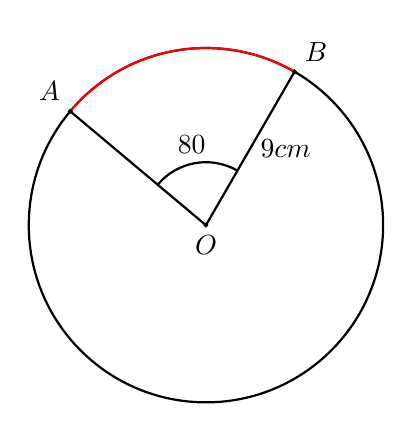
\begin{tikzpicture}[scale=0.25, >=stealth, thick]
        \coordinate (O) at (0,0);
        \coordinate (A) at (140:9);
        \coordinate (B) at (60:9);

        \draw[thick] (0,0) circle (9);
        \draw[thick] (O) -- (A);
        \draw[thick] (O) -- (B);
        \draw[thick, red] (A) arc (140:60:9);

        \filldraw (O) circle (1.5pt) node[below] {$O$};
        \filldraw (A) circle (1.5pt) node[above left] {$A$};
        \filldraw (B) circle (1.5pt) node[above right] {$B$};

        \pic [draw, "$80°$", angle eccentricity=1.3, angle radius=8mm] {angle = B--O--A};
        \node[right] at ($(O)!0.5!(B)$) {$9cm$};
    \end{tikzpicture}
\end{center}
 \paren[B]
    \begin{choices}
        \item $6.28$ cm
        \item $12.56$ cm
        \item $25.12$ cm
        \item $56.52$ cm
    \end{choices}
\end{question}

\begin{solution}
    \textbf{解析：} \\
    弧长公式：
    \[ \displaystyle l = \frac{\theta}{360°} \times 2\pi r \]
    代入 $\theta = 80°$，$r = 9$，$\pi = 3.14$：
    \[ \displaystyle l = \frac{80}{360} \times 2 \times 3.14 \times 9 \]
    先计算 $\dfrac{80}{360} = \dfrac{2}{9}$：
    \[ \displaystyle l = \frac{2}{9} \times 56.52 \]
    \[ \displaystyle = 12.56 \text{ cm} \]
    逐一排除干扰项：
    \begin{itemize}
        \item[A.] $6.28$ cm——约分时把 $\dfrac{80}{360}$ 误算成 $\dfrac{1}{9}$（应为 $\dfrac{2}{9}$），少算一倍。
        \item[C.] $25.12$ cm——把 $\dfrac{80}{360}$ 误算成 $\dfrac{4}{9}$，计算偏大一倍。
        \item[D.] $56.52$ cm——直接用圆的周长 $2\pi r = 2\times3.14\times9=56.52$ 作答，忘记乘以圆心角占比 $\dfrac{80}{360}$。
    \end{itemize}
    故选 B。
\end{solution}
%endregion


% %region 范围：信息科学与初等代数 | 考点：八进制转换为十进制 | 难度：基础
% \begin{question}
%     将八进制数 $356_{8}$ 转换为十进制数，其结果为 \paren[B]
    
%     \begin{choices}
%         \item $236$
%         \item $238$
%         \item $242$
%         \item $246$
%     \end{choices}
% \end{question}

% \begin{solution}
%     \textbf{解析：} \\
%     步骤 1：理解进位计数制中的按权展开法。\\
%     八进制数是以 $8$ 为底数的计数制度，从右往左数，各位的权重依次为 $8^0, 8^1, 8^2, \dots$
    
%     步骤 2：对八进制数 $356_{8}$ 进行按权展开求和：
%     \[ \displaystyle 356_{8} = 3 \times 8^2 + 5 \times 8^1 + 6 \times 8^0 \]
%     \[ \displaystyle = 3 \times 64 + 5 \times 8 + 6 \times 1 \]
%     \[ \displaystyle = 192 + 40 + 6 = 238 \]
%     因此，八进制数 $356_{8}$ 对应的十进制数为 $238$。

%     步骤 3：干扰项分析。\\
%     选项 A（$236$）的错误在于将个位数权值误算或最后加和时漏加了 $2$；\\
%     选项 C（$242$）和选项 D（$246$）通常是因为将 $8^2$ 错误地口算为 $66$ 或 $68$ 产生的计算失误。\\
    
%     故选 B。
% \end{solution}
% %endregion

%region
% 范围：初中代数 - 一元一次方程应用题 | 考点：年龄问题、列方程解应用题 | 难度：中等
% \begin{question}
%     父亲现年 $40$ 岁，儿子现年 $10$ 岁。几年后，父亲的年龄将是儿子年龄的 $3$ 倍？ \paren[A]
%     \begin{choices}
%         \item $5$ 年后
%         \item $10$ 年后
%         \item $15$ 年后
%         \item $20$ 年后
%     \end{choices}
% \end{question}

% \begin{solution}
%     \textbf{解析：} \\
%     设 $x$ 年后父亲的年龄是儿子的 $3$ 倍，则：
%     \[ \displaystyle 40 + x = 3(10 + x) \]
%     展开并移项：
%     \[ \displaystyle 40 + x = 30 + 3x \implies 40 - 30 = 3x - x \implies 10 = 2x \implies x = 5 \]
%     检验：$5$ 年后，父 $45$ 岁，子 $15$ 岁，$45 = 3 \times 15$，符合题意。 \\
%     逐一排除干扰项：
%     \begin{itemize}
%         \item[B.] $10$——列式时漏掉儿子年龄中的未知数 $x$（误设 $40+x=3\times10$），导致结果偏大。
%         \item[C.] $15$——移项或合并同类项时把系数 $2$ 误算成 $1$，运算错误所致。
%         \item[D.] $20$——把方程中 "$3$ 倍" 误理解为父亲比儿子大 $3$ 倍的差值直接计算，概念混淆导致的错误结果。
%     \end{itemize}
%     故选 A。
% \end{solution}

% % 范围：初中代数 - 二元一次方程组应用题 | 考点：数字问题、十位与个位关系 | 难度：中等偏难
% \begin{question}
%     一个两位数，十位数字与个位数字之和为 $11$。若将十位数字与个位数字对调，
%     所得新两位数比原两位数大 $63$，求原两位数。 \paren[B]
%     \begin{choices}
%         \item $20$
%         \item $29$
%         \item $38$
%         \item $92$
%     \end{choices}
% \end{question}

% \begin{solution}
%     \textbf{解析：} \\
%     设原两位数的十位数字为 $x$，则个位数字为 $(11-x)$。 \\
%     原两位数为：
%     \[ \displaystyle 10x + (11-x) = 9x + 11 \]
%     对调后的新两位数为：
%     \[ \displaystyle 10(11-x) + x = 110 - 9x \]
%     根据题意，新数比原数大 $63$：
%     \[ \displaystyle (110 - 9x) - (9x + 11) = 63 \]
%     化简：
%     \[ \displaystyle 99 - 18x = 63 \implies 18x = 36 \implies x = 2 \]
%     十位数字为 $2$，个位数字为 $11 - 2 = 9$，原两位数为 $29$。 \\
%     检验：对调后为 $92$，$92 - 29 = 63$，符合题意。 \\
%     逐一排除干扰项：
%     \begin{itemize}
%         \item[D.] $92$——把"对调后的新数"误当作题目所求的"原数"，问题理解方向搞反。
%         \item[C.] $38$——求出十位数字 $x=2$ 后，个位数字计算错误（误算成 $11-2=8$ 而非 $9$）。
%         \item[A.] $20$——只求出十位数字 $x=2$ 便直接作答，漏加个位数字 $9$。
%     \end{itemize}
%     故选 B。
% \end{solution}

% % 范围：初中代数 - 一元一次方程（分式方程）| 考点：去分母解方程 | 难度：中等
% \begin{question}
%     解方程 $\dfrac{2x-1}{3} - \dfrac{x+1}{2} = 1$，求 $x$ 的值。 \paren[D]
%     \begin{choices}
%         \item $1$
%         \item $6$
%         \item $7$
%         \item $11$
%     \end{choices}
% \end{question}

% \begin{solution}
%     \textbf{解析：} \\
%     方程两边同乘以最小公倍数 $6$，去分母：
%     \[ \displaystyle 6 \times \frac{2x-1}{3} - 6 \times \frac{x+1}{2} = 6 \times 1 \]
%     \[ \displaystyle 2(2x-1) - 3(x+1) = 6 \]
%     展开：
%     \[ \displaystyle 4x - 2 - 3x - 3 = 6 \]
%     合并同类项：
%     \[ \displaystyle x - 5 = 6 \implies x = 11 \]
%     检验：$\dfrac{2(11)-1}{3} - \dfrac{11+1}{2} = \dfrac{21}{3} - \dfrac{12}{2} = 7 - 6 = 1$，符合题意。 \\
%     逐一排除干扰项：
%     \begin{itemize}
%         \item[B.] $6$——去分母时只处理了左边两个分式，右边的常数 $1$ 忘记同乘 $6$，方程变为 $x-5=1$。
%         \item[A.] $1$——移项时符号出错，把 $x-5=6$ 误算成 $x=6-5$，减法与加法混淆。
%         \item[C.] $7$——展开 $-3(x+1)$ 时漏看括号内 $-2$ 的负号，误将 $4x-2-3x-3$ 算成 $4x+2-3x-3$。
%     \end{itemize}
%     故选 D。
%\end{solution}

%endregion 



\vfill % 与上方内容保持距离

\noindent
\newlength{\sigwidth}
\settowidth{\sigwidth}{（\hspace{4em}师）}

\begin{tabular*}{\textwidth}{@{\extracolsep{\fill}} l l l}
    出题： & 审题： & 审核： \\[4em]
    \rule{\sigwidth}{0.5pt} &
    \rule{\sigwidth}{0.5pt} &
    \rule{\sigwidth}{0.5pt} \\
    （\hspace{0em} \setterteacher ） &
    （\hspace{0em} \reviewteacher ） &
    （\hspace{0em} \auditteacher ） \\
\end{tabular*}


\newpage

\begin{center}
\textbf{参考答案}

\begin{tikzpicture}
  \pgfmathtruncatemacro{\cols}{ifthenelse(\answerkeytotal<=16,8,10)}
  \pgfmathsetlengthmacro{\boxw}{(\linewidth-0.4pt)/\cols}
  \pgfmathsetlengthmacro{\boxh}{1.2cm}
  \pgfmathsetlengthmacro{\offset}{0.15cm}

  \answerkeyitems
\end{tikzpicture}
\end{center}

\end{document}